%%%%%%%%%%%%%%%%%%%%%%%%
%                                                                       %
% Verification and Validation   %
%                                                                        %
%%%%%%%%%%%%%%%%%%%%%%%%%

\chapter{Verification and Validation}

During the development of this work, we have always been in contact with geochemists to present them the partial results of our geochemical speciation modelling software. We collected feedbacks regarding how to achieve a better software, as well as checking if our solution is fulfilling its purpose with consistent results. \\
As final evaluation of this work, we selected an application relevant to petroleum systems. Many physical-chemical reactions happens during the generation, migration and storage of oil. \emph{Diagenesis} is the definition of the several processes that are involved and it is driven by multiple factors as temperature, pressure, mineral composition, water composition, activity of the solutes, pH, etc. 
The \emph{diagenesis} is responsible for compaction and precipitation of minerals \cite{Tucker:01} and therefore, porosity, solubility and permeability of these reservoirs. The study of diagenesis is important because it allows to understand the geologic history of rocks, specially sedimentary rocks. In sedimentary rocks, the deposition of sediments are compacted in different layers and cemented by minerals that precipitate from reactions in a chemically very active environment. The \emph{diagenesis} reactions happens because the components are always trying to reach equilibrium, and therefore, they tend to interact with each others \cite{Burley:85}.
Using geochemical modelling softwares is a powerful tool to understand the diagenetic processes and the natural conditions that occur in this natural environment. The goal is to numerically model this environment and analyse the results of the diagenetic reactions with a petrographic analysis of the modeled reservoirs.

\section{Case Study}
We reproduce the diagenetic reactions observed in Snorre Field reservoir sandstones, Norwegian's North Sea. Morad \cite{Morad:90} describes the texture, origin, chemistry of the sandstones reservoirs in terms of the water composition and temperature. With the help and the results from this study, we  can verify \emph{SHPECK}'s results from two perspectives:
\begin{itemize}
    \item Experimentally: Morad examined two hundred representative core samples with standard optical microscopy and petrographically described the reservoirs. This analysis confirm that the our geochemical model suits the natural environment's reality;
    \item Computationally: The descriptions presented in \cite{Morad:90} of the diagenetic reactions that take place in the Snorre Field allows us to generate a comparative study. We model and compare the same environment using \emph{SHPECK}, \emph{PHREEQC} and \emph{MINTEQA2}. The water composition is detailed in \cite{Nordstrom:79};
\end{itemize}

\subsection{Experimentally validation of Shpeck}
As stated in \cite{Morad:90}, the model presented in \cite{Egeberg:88} calculates activities of the various ions of formations waters using ion association model (originally described in \cite{Wigley:77}). The thermodynamics data used are given in \cite{Helgeson:74a,  Helgeson:74b, Helgeson:76, Waltter:77, Helgeson:78, Helgeson:81}.

After studying the composition of formations waters, the goal is to demonstrate what characteristics do the components of that water adopt. This is possible by generating and analysing the graph, in this case, expressed as a function of temperature and the log activity ratio of Potassium to Sodium ions - this can be verified in details in \cite{Aagaard:89}. 

Figure ~\ref{fig:tempXactratio} brings the graph using the results from \emph{SHPECK}. It is consistent with \cite{Aagaard:89} and analysed in \cite{Morad:90}. The pattern detected is as the temperature rises and greater burial depths, the potassium activity gets higher over sodium's.

\begin{figure}[ht!]
\centering
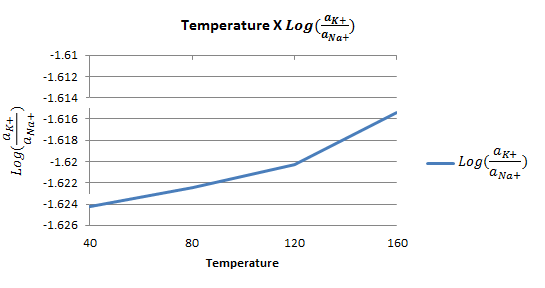
\includegraphics[width=100mm]{figures/tempXactratio.png}
\caption{Equilibrium diagram using the results from \emph{SHPECK}}
\label{fig:tempXactratio}
\end{figure}

% QUESTION:
% LEO: I wasn't sure if I should put the figure from aagaard's in order to really prove that our results are consistent.... 

\subsection{Computationally comparative} 
By modelling the same environment using three different software, we achieve a relevant comparison among the numerical methods and algorithms. 

The environment modelled is described in \cite{Morad:90} and the chemical composition of the water in \cite{Nordstrom:79}. The latter provides an analogous chemical composition of the initial solution for the sea water. It can be verified the major components in table ~\ref{tab:nordstrom} - in $mM/L$. To have an interesting and broad study the temperature range goes from $25^o$C to $160^o$C.

\begin{table}
\caption{Chemical composition of the solution in the sea water at $25^o$C }
\label{tab:nordstrom}
\centering
\begin{tabular}{r|c|c|c|c|c|c|c|c|c}
\ce{Al^{3+}} & \ce{K^+} & \ce{Na^+} & \ce{Ca^{2+}} & \ce{Mg^{2+}} & \ce{Fe^{2+}} & \ce{SiO_2}&  
\ce{SO_4^{2-}} & \ce{Cl^-} & pH
    \\ \hline
7.59e-5 & 10.45 & 479.32 & 10.53 & 54.39 & 3.66e-5 & 0.073 & 28.893 & 559.5 & 8.22
\end{tabular}
\end{table}



\section{Database Evaluation}
The database is the source of every information inside a geochemical modelling software. The goal of this section is to make clear the difference and the benefits of \emph{SHPECK}'s relational database if compared to others. In geochemical modelling software the common approach is to use flat file databases; therefore, we're going to implement a time, space and expressiveness analysis between the \emph{LLNL} thermodynamic dataset and \emph{SHPECK}'s databse. 


\subsection{Response Time analysis}
The response time is considered the sum of the processing time and the time waiting for the availabilit of the resource. It is fundamental for the performance of a geochemical modelling software to have fast access to the information since it is a bottleneck for the whole system. 
It is necessary to understand that until the software has received all the information from the database - elements, species, compounds, reactions, and so on - it will be actually doing nothing, completely stopped. This waste of CPU usage if scaled to multiple simulations and long processing is definitely something that can not be ignored. 
In order to analyze the response time, we perform database searches to retrieve the same information. The results can be seen in figure XXXXXXXXXX.

FIGURA 1 
%fetching an specie%

FIGURA 2
%fetching a reaction%

FIGURA 3
%fetching a list of compounds%

\subsection{Size and Growth analysis}
In the size analysis we compare the flat file database and a \emph{SQLite} relational database regarding the size that it takes - either from the memory and from the hard disk. Also connected to the size of the database, we have a comparative study on how to insert one information once this database has already been finished and is in use.
In order to analyse the size, we have table XXXXXXXXXXXXX.

\subsection{Expressiveness analysis}
The more expressiveness the database has, the more it provides for the system that is using it (in all possible ways). With flat file database, we have regular access to the information that it contains. In relation databases we use the \emph{SQL}. The studies in expressive power of query languages is one of the important fields in database studies - it studies the limitation and, on the other hand, the power of \emph{SQL}. Due to this works scope, we will not address basic knowledges in \emph{SQL} queries. 
In order to analyze the expressiveness, we explain how the same information needs to be requested in a flat file database and in a \emph{SQL} relational database. 

\begin{enumerate}
    \item Example 1
    \item Example 2
\end{enumerate}


\begin{itemize}
    \item Diagenetic Reactions:
    \item Verification: 
    \item Validation: 
    \item 
\end{itemize}